\documentclass{report}

\documentclass[12pt]{article}
\usepackage{array}
\usepackage{color}
\usepackage{amsthm}
\usepackage{eufrak}
\usepackage{lipsum}
\usepackage{pifont}
\usepackage{yfonts}
\usepackage{amsmath}
\usepackage{amssymb}
\usepackage{ccfonts}
\usepackage{comment} \usepackage{amsfonts}
\usepackage{fancyhdr}
\usepackage{graphicx}
\usepackage{listings}
\usepackage{mathrsfs}
\usepackage{setspace}
\usepackage{textcomp}
\usepackage{blindtext}
\usepackage{enumerate}
\usepackage{microtype}
\usepackage{xfakebold}
\usepackage{kantlipsum}
%\usepackage{draftwatermark}
\usepackage[spanish]{babel}
\usepackage[margin=1.5cm, top=2cm, bottom=2cm]{geometry}
\usepackage[framemethod=tikz]{mdframed}
\usepackage[colorlinks=true,citecolor=blue,linkcolor=red,urlcolor=magenta]{hyperref}

%//////////////////////////////////////////////////////
% Watermark configuration
%//////////////////////////////////////////////////////
%\SetWatermarkScale{4}
%\SetWatermarkColor{black}
%\SetWatermarkLightness{0.95}
%\SetWatermarkText{\texttt{Watermark}}

%//////////////////////////////////////////////////////
% Frame configuration
%//////////////////////////////////////////////////////
\newmdenv[tikzsetting={draw=gray,fill=white,fill opacity=0},backgroundcolor=none]{Frame}

%//////////////////////////////////////////////////////
% Font style configuration
%//////////////////////////////////////////////////////
\renewcommand{\familydefault}{\ttdefault}
\renewcommand{\rmdefault}{tt}

%//////////////////////////////////////////////////////
% Bold configuration
%//////////////////////////////////////////////////////
\newcommand{\fbseries}{\unskip\setBold\aftergroup\unsetBold\aftergroup\ignorespaces}
\makeatletter
\newcommand{\setBoldness}[1]{\def\fake@bold{#1}}
\makeatother

%//////////////////////////////////////////////////////
% Default font configuration
%//////////////////////////////////////////////////////
\DeclareFontFamily{\encodingdefault}{\ttdefault}{%
  \hyphenchar\font=\defaulthyphenchar
  \fontdimen2\font=0.33333em
  \fontdimen3\font=0.16667em
  \fontdimen4\font=0.11111em
  \fontdimen7\font=0.11111em}


%From M275 "Topology" at SJSU
\newcommand{\id}{\mathrm{id}}
\newcommand{\taking}[1]{\xrightarrow{#1}}
\newcommand{\inv}{^{-1}}

%From M170 "Introduction to Graph Theory" at SJSU
\DeclareMathOperator{\diam}{diam}
\DeclareMathOperator{\ord}{ord}
\newcommand{\defeq}{\overset{\mathrm{def}}{=}}

%From the USAMO .tex files
\newcommand{\ts}{\textsuperscript}
\newcommand{\dg}{^\circ}
\newcommand{\ii}{\item}

% % From Math 55 and Math 145 at Harvard
% \newenvironment{subproof}[1][Proof]{%
% \begin{proof}[#1] \renewcommand{\qedsymbol}{$\blacksquare$}}%
% {\end{proof}}

\newcommand{\liff}{\leftrightarrow}
\newcommand{\lthen}{\rightarrow}
\newcommand{\opname}{\operatorname}
\newcommand{\surjto}{\twoheadrightarrow}
\newcommand{\injto}{\hookrightarrow}
\newcommand{\On}{\mathrm{On}} % ordinals
\DeclareMathOperator{\img}{im} % Image
\DeclareMathOperator{\Img}{Im} % Image
\DeclareMathOperator{\coker}{coker} % Cokernel
\DeclareMathOperator{\Coker}{Coker} % Cokernel
\DeclareMathOperator{\Ker}{Ker} % Kernel
\DeclareMathOperator{\rank}{rank}
\DeclareMathOperator{\Spec}{Spec} % spectrum
\DeclareMathOperator{\Tr}{Tr} % trace
\DeclareMathOperator{\pr}{pr} % projection
\DeclareMathOperator{\ext}{ext} % extension
\DeclareMathOperator{\pred}{pred} % predecessor
\DeclareMathOperator{\dom}{dom} % domain
\DeclareMathOperator{\ran}{ran} % range
\DeclareMathOperator{\Hom}{Hom} % homomorphism
\DeclareMathOperator{\Mor}{Mor} % morphisms
\DeclareMathOperator{\End}{End} % endomorphism

\newcommand{\eps}{\epsilon}
\newcommand{\veps}{\varepsilon}
\newcommand{\ol}{\overline}
\newcommand{\ul}{\underline}
\newcommand{\wt}{\widetilde}
\newcommand{\wh}{\widehat}
\newcommand{\vocab}[1]{\textbf{\color{blue} #1}}
\providecommand{\half}{\frac{1}{2}}
\newcommand{\dang}{\measuredangle} %% Directed angle
\newcommand{\ray}[1]{\overrightarrow{#1}}
\newcommand{\seg}[1]{\overline{#1}}
\newcommand{\arc}[1]{\wideparen{#1}}
\DeclareMathOperator{\cis}{cis}
\DeclareMathOperator*{\lcm}{lcm}
\DeclareMathOperator*{\argmin}{arg min}
\DeclareMathOperator*{\argmax}{arg max}
\newcommand{\cycsum}{\sum_{\mathrm{cyc}}}
\newcommand{\symsum}{\sum_{\mathrm{sym}}}
\newcommand{\cycprod}{\prod_{\mathrm{cyc}}}
\newcommand{\symprod}{\prod_{\mathrm{sym}}}
\newcommand{\Qed}{\begin{flushright}\qed\end{flushright}}
\newcommand{\parinn}{\setlength{\parindent}{1cm}}
\newcommand{\parinf}{\setlength{\parindent}{0cm}}
% \newcommand{\norm}{\|\cdot\|}
\newcommand{\inorm}{\norm_{\infty}}
\newcommand{\opensets}{\{V_{\alpha}\}_{\alpha\in I}}
\newcommand{\oset}{V_{\alpha}}
\newcommand{\opset}[1]{V_{\alpha_{#1}}}
\newcommand{\lub}{\text{lub}}
\newcommand{\del}[2]{\frac{\partial #1}{\partial #2}}
\newcommand{\Del}[3]{\frac{\partial^{#1} #2}{\partial^{#1} #3}}
\newcommand{\deld}[2]{\dfrac{\partial #1}{\partial #2}}
\newcommand{\Deld}[3]{\dfrac{\partial^{#1} #2}{\partial^{#1} #3}}
\newcommand{\lm}{\lambda}
\newcommand{\uin}{\mathbin{\rotatebox[origin=c]{90}{$\in$}}}
\newcommand{\usubset}{\mathbin{\rotatebox[origin=c]{90}{$\subset$}}}
\newcommand{\lt}{\left}
\newcommand{\rt}{\right}
\newcommand{\paren}[1]{\left(#1\right)}
\newcommand{\bs}[1]{\boldsymbol{#1}}
\newcommand{\exs}{\exists}
\newcommand{\st}{\strut}
\newcommand{\dps}[1]{\displaystyle{#1}}

\newcommand{\sol}{\setlength{\parindent}{0cm}\textbf{\textit{Solution:}}\setlength{\parindent}{1cm} }
\newcommand{\solve}[1]{\setlength{\parindent}{0cm}\textbf{\textit{Solution: }}\setlength{\parindent}{1cm}#1 \Qed}

% Things Lie
\newcommand{\kb}{\mathfrak b}
\newcommand{\kg}{\mathfrak g}
\newcommand{\kh}{\mathfrak h}
\newcommand{\kn}{\mathfrak n}
\newcommand{\ku}{\mathfrak u}
\newcommand{\kz}{\mathfrak z}
\DeclareMathOperator{\Ext}{Ext} % Ext functor
\DeclareMathOperator{\Tor}{Tor} % Tor functor
\newcommand{\gl}{\opname{\mathfrak{gl}}} % frak gl group
\renewcommand{\sl}{\opname{\mathfrak{sl}}} % frak sl group chktex 6

% More script letters etc.
\newcommand{\SA}{\mathcal A}
\newcommand{\SB}{\mathcal B}
\newcommand{\SC}{\mathcal C}
\newcommand{\SF}{\mathcal F}
\newcommand{\SG}{\mathcal G}
\newcommand{\SH}{\mathcal H}
\newcommand{\OO}{\mathcal O}

\newcommand{\SCA}{\mathscr A}
\newcommand{\SCB}{\mathscr B}
\newcommand{\SCC}{\mathscr C}
\newcommand{\SCD}{\mathscr D}
\newcommand{\SCE}{\mathscr E}
\newcommand{\SCF}{\mathscr F}
\newcommand{\SCG}{\mathscr G}
\newcommand{\SCH}{\mathscr H}

% Mathfrak primes
\newcommand{\km}{\mathfrak m}
\newcommand{\kp}{\mathfrak p}
\newcommand{\kq}{\mathfrak q}

% number sets
\newcommand{\RR}[1][]{\ensuremath{\ifstrempty{#1}{\mathbb{R}}{\mathbb{R}^{#1}}}}
\newcommand{\NN}[1][]{\ensuremath{\ifstrempty{#1}{\mathbb{N}}{\mathbb{N}^{#1}}}}
\newcommand{\ZZ}[1][]{\ensuremath{\ifstrempty{#1}{\mathbb{Z}}{\mathbb{Z}^{#1}}}}
\newcommand{\QQ}[1][]{\ensuremath{\ifstrempty{#1}{\mathbb{Q}}{\mathbb{Q}^{#1}}}}
\newcommand{\CC}[1][]{\ensuremath{\ifstrempty{#1}{\mathbb{C}}{\mathbb{C}^{#1}}}}
\newcommand{\PP}[1][]{\ensuremath{\ifstrempty{#1}{\mathbb{P}}{\mathbb{P}^{#1}}}}
\newcommand{\HH}[1][]{\ensuremath{\ifstrempty{#1}{\mathbb{H}}{\mathbb{H}^{#1}}}}
\newcommand{\FF}[1][]{\ensuremath{\ifstrempty{#1}{\mathbb{F}}{\mathbb{F}^{#1}}}}
% expected value
\newcommand{\EE}{\ensuremath{\mathbb{E}}}
\newcommand{\charin}{\text{ char }}
\DeclareMathOperator{\sign}{sign}
\DeclareMathOperator{\Aut}{Aut}
\DeclareMathOperator{\Inn}{Inn}
\DeclareMathOperator{\Syl}{Syl}
\DeclareMathOperator{\Gal}{Gal}
\DeclareMathOperator{\GL}{GL} % General linear group
\DeclareMathOperator{\SL}{SL} % Special linear group

%---------------------------------------
% BlackBoard Math Fonts :-
%---------------------------------------

%Captital Letters
\newcommand{\bbA}{\mathbb{A}}	\newcommand{\bbB}{\mathbb{B}}
\newcommand{\bbC}{\mathbb{C}}	\newcommand{\bbD}{\mathbb{D}}
\newcommand{\bbE}{\mathbb{E}}	\newcommand{\bbF}{\mathbb{F}}
\newcommand{\bbG}{\mathbb{G}}	\newcommand{\bbH}{\mathbb{H}}
\newcommand{\bbI}{\mathbb{I}}	\newcommand{\bbJ}{\mathbb{J}}
\newcommand{\bbK}{\mathbb{K}}	\newcommand{\bbL}{\mathbb{L}}
\newcommand{\bbM}{\mathbb{M}}	\newcommand{\bbN}{\mathbb{N}}
\newcommand{\bbO}{\mathbb{O}}	\newcommand{\bbP}{\mathbb{P}}
\newcommand{\bbQ}{\mathbb{Q}}	\newcommand{\bbR}{\mathbb{R}}
\newcommand{\bbS}{\mathbb{S}}	\newcommand{\bbT}{\mathbb{T}}
\newcommand{\bbU}{\mathbb{U}}	\newcommand{\bbV}{\mathbb{V}}
\newcommand{\bbW}{\mathbb{W}}	\newcommand{\bbX}{\mathbb{X}}
\newcommand{\bbY}{\mathbb{Y}}	\newcommand{\bbZ}{\mathbb{Z}}

%---------------------------------------
% MathCal Fonts :-
%---------------------------------------

%Captital Letters
\newcommand{\mcA}{\mathcal{A}}	\newcommand{\mcB}{\mathcal{B}}
\newcommand{\mcC}{\mathcal{C}}	\newcommand{\mcD}{\mathcal{D}}
\newcommand{\mcE}{\mathcal{E}}	\newcommand{\mcF}{\mathcal{F}}
\newcommand{\mcG}{\mathcal{G}}	\newcommand{\mcH}{\mathcal{H}}
\newcommand{\mcI}{\mathcal{I}}	\newcommand{\mcJ}{\mathcal{J}}
\newcommand{\mcK}{\mathcal{K}}	\newcommand{\mcL}{\mathcal{L}}
\newcommand{\mcM}{\mathcal{M}}	\newcommand{\mcN}{\mathcal{N}}
\newcommand{\mcO}{\mathcal{O}}	\newcommand{\mcP}{\mathcal{P}}
\newcommand{\mcQ}{\mathcal{Q}}	\newcommand{\mcR}{\mathcal{R}}
\newcommand{\mcS}{\mathcal{S}}	\newcommand{\mcT}{\mathcal{T}}
\newcommand{\mcU}{\mathcal{U}}	\newcommand{\mcV}{\mathcal{V}}
\newcommand{\mcW}{\mathcal{W}}	\newcommand{\mcX}{\mathcal{X}}
\newcommand{\mcY}{\mathcal{Y}}	\newcommand{\mcZ}{\mathcal{Z}}


%---------------------------------------
% Bold Math Fonts :-
%---------------------------------------

%Captital Letters
\newcommand{\bmA}{\boldsymbol{A}}	\newcommand{\bmB}{\boldsymbol{B}}
\newcommand{\bmC}{\boldsymbol{C}}	\newcommand{\bmD}{\boldsymbol{D}}
\newcommand{\bmE}{\boldsymbol{E}}	\newcommand{\bmF}{\boldsymbol{F}}
\newcommand{\bmG}{\boldsymbol{G}}	\newcommand{\bmH}{\boldsymbol{H}}
\newcommand{\bmI}{\boldsymbol{I}}	\newcommand{\bmJ}{\boldsymbol{J}}
\newcommand{\bmK}{\boldsymbol{K}}	\newcommand{\bmL}{\boldsymbol{L}}
\newcommand{\bmM}{\boldsymbol{M}}	\newcommand{\bmN}{\boldsymbol{N}}
\newcommand{\bmO}{\boldsymbol{O}}	\newcommand{\bmP}{\boldsymbol{P}}
\newcommand{\bmQ}{\boldsymbol{Q}}	\newcommand{\bmR}{\boldsymbol{R}}
\newcommand{\bmS}{\boldsymbol{S}}	\newcommand{\bmT}{\boldsymbol{T}}
\newcommand{\bmU}{\boldsymbol{U}}	\newcommand{\bmV}{\boldsymbol{V}}
\newcommand{\bmW}{\boldsymbol{W}}	\newcommand{\bmX}{\boldsymbol{X}}
\newcommand{\bmY}{\boldsymbol{Y}}	\newcommand{\bmZ}{\boldsymbol{Z}}
%Small Letters
\newcommand{\bma}{\boldsymbol{a}}	\newcommand{\bmb}{\boldsymbol{b}}
\newcommand{\bmc}{\boldsymbol{c}}	\newcommand{\bmd}{\boldsymbol{d}}
\newcommand{\bme}{\boldsymbol{e}}	\newcommand{\bmf}{\boldsymbol{f}}
\newcommand{\bmg}{\boldsymbol{g}}	\newcommand{\bmh}{\boldsymbol{h}}
\newcommand{\bmi}{\boldsymbol{i}}	\newcommand{\bmj}{\boldsymbol{j}}
\newcommand{\bmk}{\boldsymbol{k}}	\newcommand{\bml}{\boldsymbol{l}}
\newcommand{\bmm}{\boldsymbol{m}}	\newcommand{\bmn}{\boldsymbol{n}}
\newcommand{\bmo}{\boldsymbol{o}}	\newcommand{\bmp}{\boldsymbol{p}}
\newcommand{\bmq}{\boldsymbol{q}}	\newcommand{\bmr}{\boldsymbol{r}}
\newcommand{\bms}{\boldsymbol{s}}	\newcommand{\bmt}{\boldsymbol{t}}
\newcommand{\bmu}{\boldsymbol{u}}	\newcommand{\bmv}{\boldsymbol{v}}
\newcommand{\bmw}{\boldsymbol{w}}	\newcommand{\bmx}{\boldsymbol{x}}
\newcommand{\bmy}{\boldsymbol{y}}	\newcommand{\bmz}{\boldsymbol{z}}

%---------------------------------------
% Scr Math Fonts :-
%---------------------------------------

\newcommand{\sA}{{\mathscr{A}}}   \newcommand{\sB}{{\mathscr{B}}}
\newcommand{\sC}{{\mathscr{C}}}   \newcommand{\sD}{{\mathscr{D}}}
\newcommand{\sE}{{\mathscr{E}}}   \newcommand{\sF}{{\mathscr{F}}}
\newcommand{\sG}{{\mathscr{G}}}   \newcommand{\sH}{{\mathscr{H}}}
\newcommand{\sI}{{\mathscr{I}}}   \newcommand{\sJ}{{\mathscr{J}}}
\newcommand{\sK}{{\mathscr{K}}}   \newcommand{\sL}{{\mathscr{L}}}
\newcommand{\sM}{{\mathscr{M}}}   \newcommand{\sN}{{\mathscr{N}}}
\newcommand{\sO}{{\mathscr{O}}}   \newcommand{\sP}{{\mathscr{P}}}
\newcommand{\sQ}{{\mathscr{Q}}}   \newcommand{\sR}{{\mathscr{R}}}
\newcommand{\sS}{{\mathscr{S}}}   \newcommand{\sT}{{\mathscr{T}}}
\newcommand{\sU}{{\mathscr{U}}}   \newcommand{\sV}{{\mathscr{V}}}
\newcommand{\sW}{{\mathscr{W}}}   \newcommand{\sX}{{\mathscr{X}}}
\newcommand{\sY}{{\mathscr{Y}}}   \newcommand{\sZ}{{\mathscr{Z}}}


%---------------------------------------
% Math Fraktur Font
%---------------------------------------

%Captital Letters
\newcommand{\mfA}{\mathfrak{A}}	\newcommand{\mfB}{\mathfrak{B}}
\newcommand{\mfC}{\mathfrak{C}}	\newcommand{\mfD}{\mathfrak{D}}
\newcommand{\mfE}{\mathfrak{E}}	\newcommand{\mfF}{\mathfrak{F}}
\newcommand{\mfG}{\mathfrak{G}}	\newcommand{\mfH}{\mathfrak{H}}
\newcommand{\mfI}{\mathfrak{I}}	\newcommand{\mfJ}{\mathfrak{J}}
\newcommand{\mfK}{\mathfrak{K}}	\newcommand{\mfL}{\mathfrak{L}}
\newcommand{\mfM}{\mathfrak{M}}	\newcommand{\mfN}{\mathfrak{N}}
\newcommand{\mfO}{\mathfrak{O}}	\newcommand{\mfP}{\mathfrak{P}}
\newcommand{\mfQ}{\mathfrak{Q}}	\newcommand{\mfR}{\mathfrak{R}}
\newcommand{\mfS}{\mathfrak{S}}	\newcommand{\mfT}{\mathfrak{T}}
\newcommand{\mfU}{\mathfrak{U}}	\newcommand{\mfV}{\mathfrak{V}}
\newcommand{\mfW}{\mathfrak{W}}	\newcommand{\mfX}{\mathfrak{X}}
\newcommand{\mfY}{\mathfrak{Y}}	\newcommand{\mfZ}{\mathfrak{Z}}
%Small Letters
\newcommand{\mfa}{\mathfrak{a}}	\newcommand{\mfb}{\mathfrak{b}}
\newcommand{\mfc}{\mathfrak{c}}	\newcommand{\mfd}{\mathfrak{d}}
\newcommand{\mfe}{\mathfrak{e}}	\newcommand{\mff}{\mathfrak{f}}
\newcommand{\mfg}{\mathfrak{g}}	\newcommand{\mfh}{\mathfrak{h}}
\newcommand{\mfi}{\mathfrak{i}}	\newcommand{\mfj}{\mathfrak{j}}
\newcommand{\mfk}{\mathfrak{k}}	\newcommand{\mfl}{\mathfrak{l}}
\newcommand{\mfm}{\mathfrak{m}}	\newcommand{\mfn}{\mathfrak{n}}
\newcommand{\mfo}{\mathfrak{o}}	\newcommand{\mfp}{\mathfrak{p}}
\newcommand{\mfq}{\mathfrak{q}}	\newcommand{\mfr}{\mathfrak{r}}
\newcommand{\mfs}{\mathfrak{s}}	\newcommand{\mft}{\mathfrak{t}}
\newcommand{\mfu}{\mathfrak{u}}	\newcommand{\mfv}{\mathfrak{v}}
\newcommand{\mfw}{\mathfrak{w}}	\newcommand{\mfx}{\mathfrak{x}}
\newcommand{\mfy}{\mathfrak{y}}	\newcommand{\mfz}{\mathfrak{z}}


\usepackage{float}
\usetikzlibrary{decorations.markings, calc}
\usetikzlibrary{arrows.meta}

\title{\Huge{Electro 1}\\Tarea 4}
\author{\huge{Sergio Montoya Ramirez}}
\date{}

\begin{document}

\maketitle
\newpage% or \cleardoublepage
% \pdfbookmark[<level>]{<title>}{<dest>}
\pdfbookmark[section]{\contentsname}{toc}
\tableofcontents
\pagebreak

\chapter{Punto 2}

\dfn{Fuerza de Lorentz}{
	\[ \vec{F} = q \left( \vec{E} + \vec{v} \times \vec{B} \right) \]
}

\section{}

\begin{align*}
	\vec{v} &= 0 \hat{x} + \dot{y} \hat{y} + z \hat{z}\\
	\vec{B} &= B_0 \hat{x} + 0 \hat{y} + 0 \hat{z}\\
	\vec{v} \times \vec{B} &= \begin{bmatrix}
		\hat{x} & \hat{y} & \hat{z}\\
		0 & \dot{y} & \dot{z} \\
		B_0 & 0 & 0
	\end{bmatrix}\\
	&= 0 \hat{x} + \dot{z}B_0 \hat{y} - \dot{y}B_0 \hat{z}\\
	&= \dot{z}B_0 \hat{y} - \dot{y}B_0 \hat{z}\\
	\vec{F} &= Q \left( \vec{E} + \vec{v} \times \vec{B} \right)\\
	\vec{F} &= Q \left( E_0 \hat{z} + \dot{z}B_0 \hat{y} - \dot{y}B_0 \hat{z} \right)\\
	\vec{F_x} &= 0\\
	\vec{F_y} &= Q \dot{z}B_0 \hat{y}\\
	\vec{F_z} &= Q \left( E_0 - \dot{y}B_0 \right) \hat{z}\\
	m \ddot{x} &= 0\\
	m \ddot{y} &= Q \dot{z}B_0 \hat{y}\\
	m \ddot{z} &= Q \left( E_0 - \dot{y}B_0 \right) \hat{z}
\end{align*}

Con esto entonces tenemos:
\begin{align*}
	\ddot{z} + \frac{Q B_0}{m}\dot{y} - \frac{Q E_0}{m} &= 0\\
	\omega &= \frac{Q B_0}{m}\\
	\ddot{z} + \omega \dot{y} - \omega \frac{E_0}{B_0} &= 0\\
	\ddot{z} + \omega \left(\dot{y} - \frac{E_0}{B_0} \right) &= 0\\
\end{align*}

Y tambien:
\begin{align*}
	\ddot{y} - \frac{Q B_0}{m} \dot{z} &= 0\\
	\omega &= \frac{Q B_0}{m}\\
	\ddot{y} - \omega \dot{z} &= 0\\
	\ddot{y} &= \omega \dot{z}\\
\end{align*}

Juntando todo:
\begin{align*}
	\dddot{y} &= \omega \ddot{z} \\
	\iff \ddot{z} &= \frac{\dddot{y}}{\omega}\\
	\ddot{z} &= \frac{\dddot{y}}{\omega}\\
	&= \omega \left( \frac{E_0}{B_0} - \dot{y} \right)\\
	\dddot{y} &= \omega^2 \left( \frac{E_0}{B_0} - \dot{y} \right)
\end{align*}

Con esto entonces:
\begin{align*}
	y(t) &= C_1 \cos \left(\omega t \right) + C_2 \sin\left( \omega t \right) + \frac{E_0}{B_0} t + C_3\\
	z(t) &= C_2 \cos \left(\omega t \right) - C_1 \sin\left( \omega t \right) + \frac{E_0}{B_0} + C_3\\
\end{align*}

Ahora lo que nos hace falta es encontrar los valores dadas las condiciones iniciales.
\begin{align*}
	\dot{y} (0) &= \dot{z} (0) = 0\\
	y(0) &= z(0) = 0
\end{align*}

Con esto entonces:
\begin{align*}
	y(0) &= C_1 \cos \left(\omega 0 \right) + C_2 \sin\left( \omega 0 \right) + \frac{E_0}{B_0} 0 + C_3\\
	y(0) &= C_1 + C_3\\
	z(0) &= C_2 \cos \left(\omega 0 \right) - C_1 \sin\left( \omega 0 \right) + C_4\\
	z(0) &= C_2 + C_4\\
	C_1 + C_3 &= C_2 + C_4\\
	\dot{y}(t) &= - C_1\omega \sin \left(\omega t \right) + C_2 \omega\cos\left( \omega t \right) + \frac{E_0}{B_0}\\
	\dot{z}(t) &= - C_2\omega \sin \left(\omega t \right) - C_1 \omega\cos\left( \omega t \right)\\
	C_2 \omega + \frac{E_0}{B_0} &= - C_1 \omega\\
	\leftrightarrow C_2 &= \frac{1}{\omega} \left( - \frac{E_0}{B_0} - C_1 \omega\right)\\
	&= - \frac{E_0}{B_0 \omega} - C_1\\
\end{align*}

Con esto entonces:
\begin{align*}
	C_1 + C_3 &= 0 \iff C_1 = - C_3\\
	C_2 \omega + \frac{E_0}{B_0} &= 0 \iff C_2 = - \frac{E_0}{\omega B_0}\\
	C_2 + C_4 &= 0\\
	C_2 &= - C_4\\
	C_4 &= \frac{E_0}{\omega B_0}
\end{align*}

Con lo cual finalmente queda:
\begin{align*}
	y(t) &= - \frac{E_0}{\omega B_0} \sin \left(\omega t\right) + \frac{E_0}{B_0} t\\
	&= \frac{E_0}{B_0 \omega} \left( \omega t - \sin \left(\omega t \right)\right)\\
	z(t) &= - \frac{E_0}{\omega B_0} \cos\left(\omega t\right) + \frac{E_0}{\omega B_0}\\
	z(t) &= \frac{E_0}{\omega B_0} \left( 1 - \cos\left(\omega t\right)\right)
\end{align*}

\section{}

Ahora con esto para encontrar el Radio tomemos
\begin{align*}
	R &= \frac{E_0}{\omega B_0}\\
	y(t) &= \frac{E_0}{B_0 \omega} \left(\omega t - \sin\left(\omega t\right)\right)\\
	- \sin \left(\omega t\right) &= \frac{B_0 \omega}{E_0} \left(y(t) - \frac{E_0 t}{B_0}\right)\\
	Z(t) &= \frac{E_0}{\omega B_0} \left(1 - \cos\left(\omega t \right)\right)\\
	- \cos\left(\omega t\right) &= \frac{\omega B_0}{E_0}\left(z(t) - \frac{E_0}{\omega B_0}\right)\\
	- \cos\left(\omega t\right) &= \frac{1}{R} \left( z(t) - R\right)\\
	\cos^2\left(\omega t\right) + \sin^2\left(\omega t\right) &= 1\\
	a^2 &= -a^2\\
	\sin^2\left(\omega t\right) + \cos^2\left(\omega t\right) &= \left(- \sin\left(\omega t\right)\right)^2 + \left(- \cos\left(\omega t\right)\right)^2\\
	\left(\frac{1}{R^2} \left(y(t) - R \omega t\right)^2\right) + \left(\frac{1}{R^2} \left(z(t) - R \right)^2\right) &= 1\\
	\left(y(t) - R\omega t\right)^2 + \left(z(t) - R\right)^2 &= R^2
\end{align*}

Con esto encontramos un circulo con radio $R$

\section{}

Este problema es en esencia el ejemplo $5.2$ de la cuarta edición del Griffiths. Por lo tanto reutilizare su dibujo para no complicarme con ello.

\begin{figure}[H]
	\begin{center}
		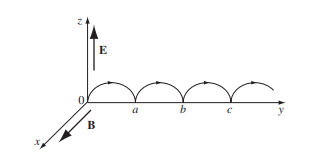
\includegraphics[width=0.45\textwidth]{img/book_5_7.png}
	\end{center}
	\caption{Dibujo del movimiento.}\label{fig:book_5_7}
\end{figure}

\chapter{Punto 3}

\section{}

El campo de una corriente es:
\dfn{Biot-Savart}{
	\[
		\vec{B}\left(\vec{r}\right) = \frac{\mu_0}{4\pi} \int \frac{\vec{I}\times \hat{r}}{r^2}dl' = \frac{\mu_0}{4\pi} I \int \frac{d\ell' \times \hat{r}}{r^2}
	\]
}

Vamos a tomar entonces este ejercicio como el de una espira cuadrada con lado $2R$

\begin{center}
	\begin{tikzpicture}[
    current direction/.style={
        decoration={
            markings,
            mark=at position 0.5 with {\arrow{latex}}
        },
        postaction={decorate}
    },
    medida/.style={|<->|, red, thick, shorten >=1mm, shorten <=1mm}
]

\def\R{1.5} % Tamaño base del sistema

% Ejes coordenados
\draw[->] (-2.5*\R,0) -- (2.5*\R,0) node[right] {$z$};
\draw[->] (0,-2.5*\R) -- (0,2.5*\R) node[above] {$y$};

% Espira cuadrada con corriente (lado izquierdo en rojo)
\draw[thick, current direction] (\R,\R) -- (-\R,\R) node[midway, above] {$I$}; % Superior
\draw[thick, red, current direction] (-\R,\R) -- (-\R,-\R); % Izquierdo (rojo)
\draw[thick, current direction] (-\R,-\R) -- (\R,-\R); % Inferior
\draw[thick, current direction] (\R,-\R) -- (\R,\R); % Derecho

% Punto central
\node[fill=red, circle, inner sep=2pt] at (0,0) {};

% Punto en lado izquierdo (a mitad de altura)
\coordinate (punto) at (-\R,0.5*\R);
\fill[red] (punto) circle (2pt);

% Línea entre centro y punto
\draw[dashed] (0,0) -- (punto);

% Triángulo rectángulo
\draw[help lines] (0,0) -- (-\R,0) -- (punto); % Lados del triángulo
\draw[medida] (-\R,0) -- node[right] {$y$} (punto); % Medida vertical
\draw[medida] (0,0) -- node[below] {$R$} (-\R,0); % Medida horizontal

% Marcas de ángulo recto
\draw[red] (-\R,0) ++(0.15,0.15) -- ++(-0.15,0) -- ++(0,-0.15);

% Etiqueta distancia

\end{tikzpicture}
\end{center}

Visto desde arriba y si lo miramos por un lado seria
\begin{center}
	\begin{tikzpicture}[scale=0.5]
  % Eje horizontal (corriente I)
  \draw[thick, ->] (-2,0) -- (5,0) node[right] {$I$};

  % Elemento de corriente dl'
  \draw[thick, ->] (3,0) -- (4,0) node[midway, above] {$d\vec{l}'$};

  % Punto P
  \fill (3,3) circle (3pt) node[above] {$P$};

  % Vector r
  \draw[thick, ->] (4,0) -- (3,3) node[midway, above right] {$\vec{r}$};

  % Línea vertical desde dl' hasta la altura de P
  \draw[dashed] (4,0) -- (4,3);

  % Ángulo theta
  \draw (4,3) -- (3.8,3) arc (90:135:0.2) node[midway, left] {$\theta$};

  % Ángulo alpha
  \draw (4,0) -- (4.2,0) arc (0:45:0.2) node[midway, right] {$\alpha$};

  % Distancia r
  \draw[dashed] (3,3) -- (3,0) node[midway, left] {$r$};

  % Distancia l'
  \draw[thick, -] (0,-0.5) -- (4,-0.5);
  \draw[thick, -|] (0,-0.7) -- (0,-0.3);
  \draw[thick, |-] (4,-0.7) -- (4,-0.3);
  \node[below] at (2,-0.5) {$l'$};

\end{tikzpicture}
\end{center}

En estos diagramas se ve que $d\ell' \times \hat{r}$ apunta hacia afuera y tiene magnitud \[
	\left|dl'\right|\left|\hat{r}\right| \sin\alpha = d\ell' \cos\theta 
\]

Ademas, podemos notar que:
\begin{align*}
	\tan\theta &= \frac{\ell'}{R} \iff \ell' = \tan\theta R\\
	\frac{d\ell'}{d\theta} &= R\frac{1}{\cos^2\theta}\\
	d\ell' &= \frac{R}{\cos^2\theta} d\theta\\
	\cos\theta &= \frac{R}{\left|\vec{r}\right|} \iff R = \left|\vec{r}\right| \cos\theta\\
	R &= r \cos\theta\\
	r &= \frac{R}{\cos\theta}\\
	\frac{1}{r^2} = \frac{\cos^2\theta}{R^2}\\
\end{align*}

Con esto
\begin{align*}
	\left|\vec{B}\left(\vec{r}\right)\right| &= \frac{\mu_0}{4\pi} \int \frac{\vec{I}\times \hat{r}}{r^2}dl' = \frac{\mu_0}{4\pi} I \int \frac{d\ell' \times \hat{r}}{r^2}\\
	&= \frac{\mu_0 I}{4\pi} \int \frac{d\ell' \cos\theta}{r^2}\\
	&= \frac{\mu_0 I}{4\pi} \int \frac{\cos^2\theta}{R^2} \cos\theta \frac{R}{\cos^2\theta} d\theta\\
	&= \frac{\mu_0 I}{4\pi} \int \frac{\cos\theta}{R} d\theta\\
	&= \frac{\mu_0 I}{4R\pi} \int \cos\theta d\theta\\
	&= \frac{\mu_0 I}{4R\pi} \left(\sin\theta_2 - \sin\theta_1\right)\\
\end{align*}

Ahora partimos la espira en cuatro segmentos y nos da:
\begin{align*}
	&= \frac{\mu_0 I}{4R\pi} \left(\sin\theta_2 - \sin\theta_1\right)\\
	&= \frac{\mu_0 I}{4R\pi} \left(\sin\frac{\pi}{4} - \sin-\frac{\pi}{4}\right)\\
	&= \frac{\mu_0 I}{4R\pi} \left(\frac{1}{\sqrt{2}} + \frac{1}{\sqrt{2}}\right)\\
	&= \frac{\mu_0 I\sqrt{2}}{4R\pi}
\end{align*}

Y en total tenemos 4 de estas secciones

\section{}

\begin{center}
	\begin{tikzpicture}[>=Stealth]
  % Punto P
  \coordinate (P) at (0,0);
  \node at (P) [below left] {$P$};

  % Radios a y b
  \draw[dashed] (P) -- (2,0) node[midway, below] {$a$};
  \draw[dashed] (P) -- ({2*cos(60)},{2*sin(60)}) node[midway, above left] {$b$};

  % Arco de radio a
  \draw[thick, ->] (2,0) arc (0:60:2);

  % Arco de radio b
  \draw[thick, ->] ({2.5*cos(60)},{2.5*sin(60)}) arc (60:0:2.5);

  % Segmento vertical izquierdo
  \draw[thick, ->] ({2.5*cos(60)},{2.5*sin(60)}) -- ({2*cos(60)},{2*sin(60)}) node[midway, left] {$I$};

  % Segmento horizontal derecho
  \draw[thick, ->] (2.5,0) -- (2,0) node[midway, below] {$I$};

  % Segmento vertical superior
  \draw[thick, ->] (0,{2.5*sin(60)}) -- (0,{2*sin(60)}) node[midway, left] {$I$};

  % Ángulo
  \draw (0.4,0) arc (0:60:0.4);

\end{tikzpicture}
\end{center}

Con esto entonces:
\begin{align*}
	\left|d\ell' \times \hat{r} \right| &= \left|d\ell'\right|\left|\hat{r}\right| \sin \left(90^{\circ}\right)\\
	\left| \vec{r}\right| &= r = R\\
	\left|\vec{B}\right| &= \frac{\mu_0 I}{4\pi} \int_{\frac{\pi}{2}}^0 \frac{\left|\vec{d\ell}'\times \hat{r}\right|}{R^2}\\
	\left|\vec{B}\right| &= \frac{\mu_0 I}{4\pi R} \int_{\theta_1}^{\theta_2} d\theta
\end{align*}

Con lo que

\begin{align*}
	\left|\vec{B}\right| &= \frac{\mu_0 I}{4\pi R} \int_{\theta_1}^{\theta_2} d\theta\\
	\left|\vec{B}\right| &= \frac{\mu_0 I}{4\pi R} \frac{\pi}{2}\\
	\left|\vec{B}\right| &= \frac{\mu_0 I}{8 R}\\
\end{align*}

\section{}

Este punto es basicamente una combinación de los anteriores.

Tenemos para las secciones rectas:
\begin{align*}
	\left| \vec{B} \right| &= \frac{\mu_0 I}{4\pi R} \left(\sin\theta_2 - \sin\theta_1\right)
\end{align*}

Con la regla de la mano derecha vemos que entra el vector
\begin{align*}
	\left| \vec{B} \right| &= \frac{\mu_0 I}{4\pi R}\left(\sin\pi - \sin 0\right)\\
	&= \frac{\mu_0 I}{4\pi R}\\
\end{align*}

En el caso del semicirculo 

\begin{align*}
	\left| \vec{B}\right| &= \frac{\mu_0 I}{4\pi R} \int_{\theta_1}^{\theta_2} d\theta\\
	&= \frac{\mu_0 I}{4 R}\left( \frac{3}{2} - \frac{1}{2}\right)\\
	&= \frac{\mu I}{4 R}
\end{align*}

Ahora sumamos todo y nos queda:
\begin{align*}
	B &= \frac{\mu_0 I}{4\pi R} + \frac{\mu_0 I}{4\pi R} + \frac{\mu I}{4 R}\\
	&= \frac{\mu_0 I}{4R} \left(\frac{2}{\pi} + 1 \right)
\end{align*}



\chapter{Punto 7}

\chapter{Punto 8}

\chapter{Punto 9}

\chapter{Punto 11}

Para este fonografo dado que rota a una velocidad angular $\omega$ tenemos
\begin{align*}
	I &= \sigma v dr\\
	&= \sigma \omega r dr
\end{align*}

Y podemos ver esto como la suma infinitesimal de pequeños arcos como:
\begin{align*}
	\mu &= \int_0^R \pi r^2 \sigma \omega r dr\\
	\mu &= \pi \sigma \omega \int_0^R r^3 dr\\
	\mu &= \pi \sigma \omega \left[ \frac{r^4}{4} \right]_0^R\\
	\mu &= \pi \sigma \omega \frac{R^4}{4} \square
\end{align*}

\chapter{Punto 12}

\section{}

Lo primero que debemos hacer para este punto es encontrar el campo magnético para una espira. Para ello, vamos a usar Biot-Savart.

\dfn{Biot-Savart}{
	\[ \vec{B} = \frac{\mu_0}{4\pi} \int \frac{I \vec{ds} \times \hat{r}}{r^2} \]
}

Ademas, este es el ejemplo $5.6$ de la sexta edición del Griffiths. Tomemos entonces su grafica para ubicarnos mejor:

\begin{figure}[h]
	\begin{center}
		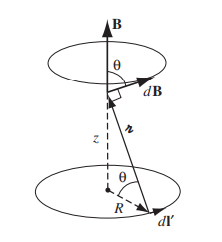
\includegraphics[width=0.25\textwidth]{img/book_5_21.png}
	\end{center}
	\caption{Figura de Representación para el problema de una espira.}\label{fig:Fig_5_21}
\end{figure}

Con esto entonces puede notar que los componentes de $d I'$ y de $d B$ se cancelan en todos los ejes excepto en el vertical en donde se suman. Por lo tanto:
\begin{align*}
	B &= \frac{\mu_0}{4\pi} \int \frac{I \vec{d s} \times \hat{r}}{r^2}\\
	B &\propto \int d B_y = \int dB \cos\theta\\
	B &= \frac{\mu_0}{4\pi} \int \frac{I \vec{d s} \sin\left(90^{\circ}\right)}{r^2}\cos\theta\\
	B &= \frac{\mu_0 I}{4\pi} \int \frac{\vec{d s}}{r^2}\cos\theta\\
	\cos\theta &= \frac{R}{\sqrt{z^2 + R^2}}\\
	r &= \sqrt{z^2 + R^2}\\
	B &= \frac{\mu_0 I}{4\pi} \int \frac{\vec{d s}}{\left(z^2 + R^2\right)}\frac{R}{\sqrt{z^2 + R^2}}\\
	B &= \frac{\mu_0 I R}{4\pi \left[ z^2 + R^2\right]^{\frac{3}{2}}} \int \vec{d s}\\
	B &= \frac{\mu_0 I R}{4\pi \left[ z^2 + R^2\right]^{\frac{3}{2}}} \left( 2\pi R\right)\\
	B &= \frac{\mu_0 I R^2}{2\left[ z^2 + R^2\right]^{\frac{3}{2}}}\\
\end{align*}

Ahora bien dado que tenemos dos espiras por superposición podemos poner:

\begin{enumerate}
	\item $$z = \frac{d}{2} + z$$
		\begin{align*}
			B_+ &= \frac{\mu_0 I R^2}{2\left[ z^2 + R^2\right]^{\frac{3}{2}}}\\
			B_+ &= \frac{\mu_0 I R^2}{2\left[ \left(\frac{d}{2} + z\right)^2 + R^2\right]^{\frac{3}{2}}}\\
		\end{align*}
	\item $$z = \frac{d}{2} - z$$
		\begin{align*}
			B_- &= \frac{\mu_0 I R^2}{2\left[ z^2 + R^2\right]^{\frac{3}{2}}}\\
			B_- &= \frac{\mu_0 I R^2}{2\left[ \left(\frac{d}{2} - z\right)^2 + R^2\right]^{\frac{3}{2}}}\\
		\end{align*}
\end{enumerate}

Con lo cual el resultado total es:
\begin{align*}
	B &= B_+ + B_-\\
	& = \frac{\mu_0 I R^2}{2\left[ \left(\frac{d}{2} + z\right)^2 + R^2\right]^{\frac{3}{2}}} + \frac{\mu_0 I R^2}{2\left[ \left(\frac{d}{2} - z\right)^2 + R^2\right]^{\frac{3}{2}}}\\
	& = \frac{\mu_0 I R^2}{2} \left[\frac{1}{\left[ \left(\frac{d}{2} + z\right)^2 + R^2\right]^{\frac{3}{2}}} + \frac{1}{\left[ \left(\frac{d}{2} - z\right)^2 + R^2\right]^{\frac{3}{2}}}\right]\\
\end{align*}

\section{}

Podemos simplemente poner este resultado con python como:
\lstinputlisting[language=Python]{./code/punto_12_b.py}

Con lo cual recibimos la siguiente grafica:

\begin{figure}[H]
	\begin{center}
		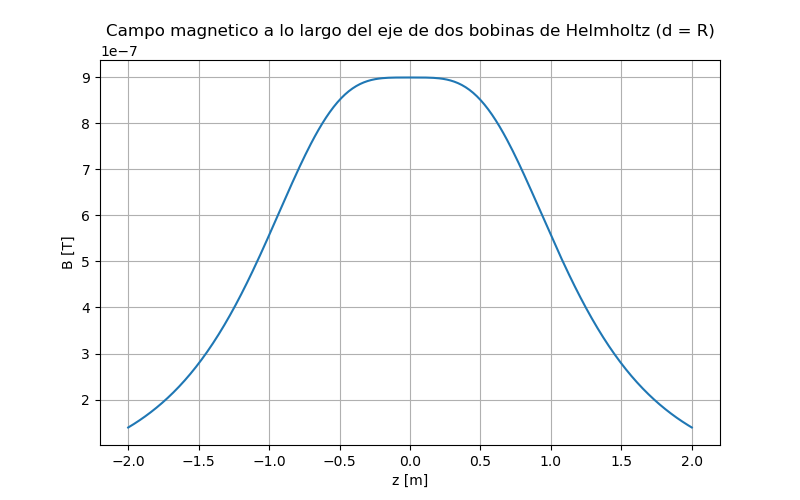
\includegraphics[width=0.75\textwidth]{img/punto_12_b.png}
	\end{center}
	\caption{Campo magnetico a lo largo del eje de dos bobinas de Helmholtz (d = R)}\label{fig:Punto_12_b}
\end{figure}

\section{}

Este punto lo podemos mirar basicamente como si esta corriente no varie mucho. Para hacer esto en esencia lo
que nos interesa es encontrar que $\frac{d^2B}{dz^2}(0) = \frac{dB}{dz}(0) = 0$ para algun $d$. Por simetria ya sabemos
que $\frac{dB}{dz}(0) = 0$. Por lo tanto solo nos queda encontrar una $d$ en la que se cumpla lo primero.

Para esto vamos a ponerlo en Sympy:
\lstinputlisting[language=Python]{./code/punto_12_c.py}

Con esto entonces podemos saber que para $B$ tenemos:
\begin{align*}
	\frac{dB}{d z}&= - \frac{24 I R^{2} \mu_{0} \left(\left(4 R^{2} + \left(d - 2 z\right)^{2}\right)^{\frac{5}{2}} \left(d + 2 z\right) - \left(4 R^{2} + \left(d + 2 z\right)^{2}\right)^{\frac{5}{2}} \left(d - 2 z\right)\right)}{\left(4 R^{2} + \left(d - 2 z\right)^{2}\right)^{\frac{5}{2}} \left(4 R^{2} + \left(d + 2 z\right)^{2}\right)^{\frac{5}{2}}}\\
	\frac{d^2 B}{d z^2} &= - \frac{48 I R^{2} \mu_{0}}{\left(4 R^{2} + \left(d + 2 z\right)^{2}\right)^{\frac{5}{2}}} + \frac{240 I R^{2} \mu_{0} \left(d + 2 z\right)^{2}}{\left(4 R^{2} + \left(d + 2 z\right)^{2}\right)^{\frac{7}{2}}} - \frac{48 I R^{2} \mu_{0}}{\left(4 R^{2} + \left(d - 2 z\right)^{2}\right)^{\frac{5}{2}}} + \frac{240 I R^{2} \mu_{0} \left(d - 2 z\right)^{2}}{\left(4 R^{2} + \left(d - 2 z\right)^{2}\right)^{\frac{7}{2}}}
\end{align*}

Ahora para solucionar podemos simplemente reemplazar $z = 0$ que nos queda como:
\[
	\frac{d^2B}{dz^2}(0) = \frac{384 I R^{2} \mu_{0} \left(- R^{2} + d^{2}\right)}{\left(4 R^{2} + d^{2}\right)^{\frac{7}{2}}}
\]

Y por ultimo bucamos un valor de $d$ para el cual
\[
	\frac{d^2B}{dz^2}(0) = 0
\]

Y nos da como resultado:
\[
	\left[ \left\{ d : R\right\}\right]
\]

Y con esto queda solucionado. Ahora veamos esta, esta bobina de Helmholtz se hace mucho mas estable cuando $d = R$ cosa que explica el por que trabajamos con ello en el punto anterior.

\section{}

Este punto es esencialmente equivalente al $A$ por lo tanto no volveremos a mirar como solucionar el campo para una espira y simplemente partiremos de antes:
\begin{align*}
	B &= B_+ + B_-\\
	& = \frac{\mu_0 I R^2}{2\left[ \left(\frac{d}{2} + z\right)^2 + R^2\right]^{\frac{3}{2}}} + \frac{\mu_0 - I R^2}{2\left[ \left(\frac{d}{2} - z\right)^2 + R^2\right]^{\frac{3}{2}}}\\
	& = \frac{\mu_0 I R^2}{2} \left[\frac{1}{\left[ \left(\frac{d}{2} + z\right)^2 + R^2\right]^{\frac{3}{2}}} - \frac{1}{\left[ \left(\frac{d}{2} - z\right)^2 + R^2\right]^{\frac{3}{2}}}\right]\\
\end{align*}

En esencia es evidente lo que estoy poniendo pues es simplemente decir que cuando las corrientes son inversas no se contribuyen si no que se restan.

\section{}

Para graficar esto vamos a reutilizar el codigo de antes simplemente cambiando un signo:

\lstinputlisting[language=Python]{./code/punto_12_e.py}

Con lo que nos queda el siguiente resultado:
\begin{figure}[H]
	\begin{center}
		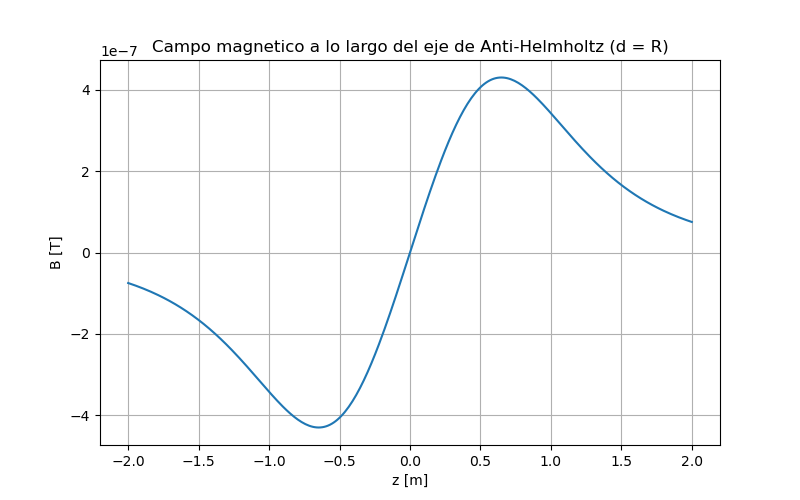
\includegraphics[width=0.95\textwidth]{img/punto_12_e.png}
	\end{center}
	\caption{Campo magnetico a lo largo del eje de Anti-Helmholtz (d = R)}\label{fig:}
\end{figure}

\section{}

Ahora vamos a buscar que en el centro $ B = - B_T$ que recordemos es aproximadamente $B_T = 50 \mu T$. Lo primero es notar que este va a ser una bobina de Helmholtz y no una antibobina pues nos interesa que en el centro sea el mayor valor y no $0$. Por lo tanto tomaremos los ejemplos anteriores.

Lo que haremos en esencia sera coger el termino anterior y reemplazarle $z = 0$ y $d = R$. Esto nos dara el resultado para $B(0)$ de una bobina de Helmholtz que queda como:
\begin{align*}
	B & = \frac{\mu_0 I R^2}{2} \left[\frac{1}{\left[ \left(\frac{d}{2} + z\right)^2 + R^2\right]^{\frac{3}{2}}} + \frac{1}{\left[ \left(\frac{d}{2} - z\right)^2 + R^2\right]^{\frac{3}{2}}}\right]\\
	B & = \frac{\mu_0 I R^2}{2} \left[\frac{1}{\left[ \left(\frac{R}{2} + 0\right)^2 + R^2\right]^{\frac{3}{2}}} + \frac{1}{\left[ \left(\frac{R}{2} - 0\right)^2 + R^2\right]^{\frac{3}{2}}}\right]\\
	B(0) &= \frac{8 \sqrt{5} I \mu_{0}}{25 R}
\end{align*}

Ahora con esto lo que nos interesa es ver cuando $B(0) = B_{tierra}$ lo cual nos permitiria despejar para la corriente y simplemente con eso ya tendriamos dado $R$ cual deberia ser la corriente que pase para que en el centro el campo terrestre se anule:

\begin{align*}
	B(0) &= \frac{8 \sqrt{5} I \mu_{0}}{25 R} = B_{tierra}\\
	B(0) &= \frac{5 \sqrt{5} B_{tierra} R}{8 \mu_{0}}
\end{align*}

Ahora ya apartir de esto podemos hacerlo tan arbitrario como  querramos.

Para mostrar esto tambien lo hice con sympy y obtuve los mismos resultados:
\lstinputlisting[language=Python]{./code/punto_12_f.py}


\end{document}
